\chapter{Réalisations}
\label{Developpement}


\section{Les Projets}

\subsection{MobiSaaS}

\subsubsection{Présentation : spécifications fonctionnelles}

Le projet "MobiSaaS" s'inscrit dans la démarche d'entreprise de proposer des solutions en mode \textbf{SAAS}. Le projet consiste d'une manière générale à exposer les fonctionnalité de la solution desktop du produit "MobiAnalyst"(Fig. \ref{OffreMobiAnalyst}).

\begin{figure}[!h]
\centering
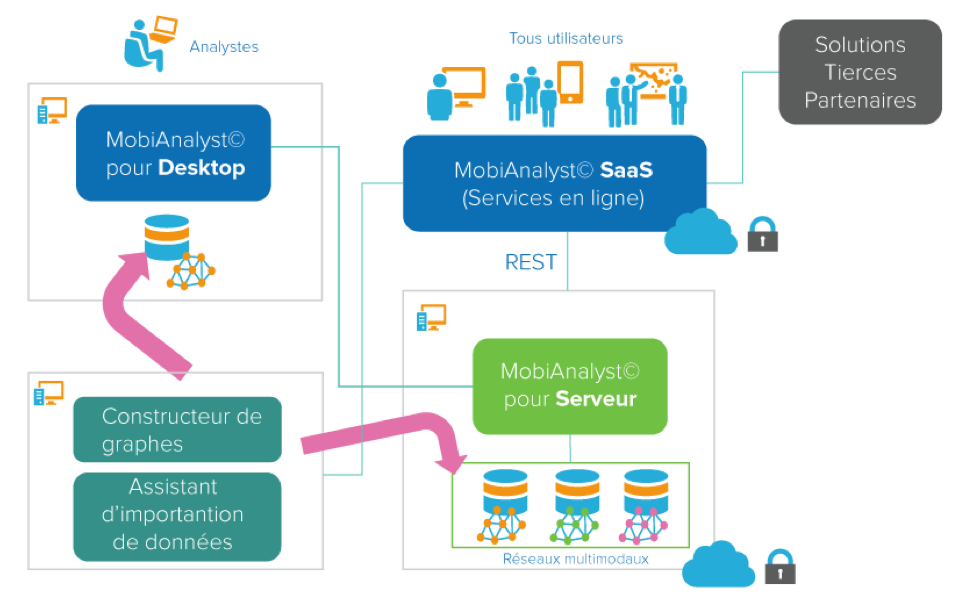
\includegraphics[width=14cm]{images/offre_MobiAnalyst.png}
\caption{\label{OffreMobiAnalyst}Offre du produit MobiAnalyst}
\end{figure} 

\subsubsection{Technologies : spécifications techniques}

Pour le projet "MobiSaaS" le choix technologique majeur est d'utiliser le framework DropWizard (cf. Annexe \ref{Annexe B}). Ce framework orienté micro-services nous permet de fournir notamment un serveur embarqué HTTP "Jetty". Jersey pour la partie webservice REST qui est l'implémentation de référence de la spécification JAX-RS. Ou encore Jakson pour la dé/sérialisation du JSON. Cette application est couplée à un serveur cartographique (ArcGIS), afin de proposer une interface cartographique.\\

L'environnement de développement est donc un projet Java EE Maven composé des éléments de Dropwizard. \\
Ces WS sont à priori “lourds”, sachant qu'un jeu de données (ex: GTFS\footnote{\url{https://developers.google.com/transit/gtfs/reference}}) fait plusieurs centaines de Mo, les opérations de téléchargement, validation, traitement, stockage dans en base,... vont être long à renvoyer une réponse au client après chaque requête. Les WS à développer sont donc asynchrones. De plus, une contrainte supplémentaire et que le service doit supporter plusieurs requêtes simultanées, il faudra donc s'orienter vers un développement en mode "programmation concurrente".\\

\subsubsection{Objectifs / Développements}

Le but de mon stage est de développer des web services WS en amont du DataWizard en mode \textbf{SAAS} (cf.définition) dont principalement l'import de données GTFS. L'objectif de ce service est de pouvoir manipuler ces données (comme le fait le DataWizard) et ainsi pouvoir récupérer des métadonnées ex: l'extension géographique des données, le nom de l'agence, le nombre de lignes, le mode de transport,...\\




\subsubsection{Résultats obtenus / Difficultés rencontrées}

J'ai tout d'abord commencé par découvrir Maven (cf. Annexe \ref{Annexe A}), les projets, les modules, le désormais célèbre fichier \textbf{POM}, etc...
Ensuite, je me suis documenté sur le code métier existant, et chercher des outils ou librairies de professionnels du domaine (cf. Outils métiers \ref{OBA}).
Enfin, après le "Getting Started" de Dropwizard\footnote{\url{https://dropwizard.github.io/dropwizard/getting-started.html}}, une fois tout cela bien maîtrisé, j'ai pu  commencé la conception et le développement de services web REST.\\

J'ai choisit de stocker les informations concernant ma partie de l'application dans une table PostgreSQL (Fig \ref{TablePostgres})\\
\begin{figure}[!h]
\centering
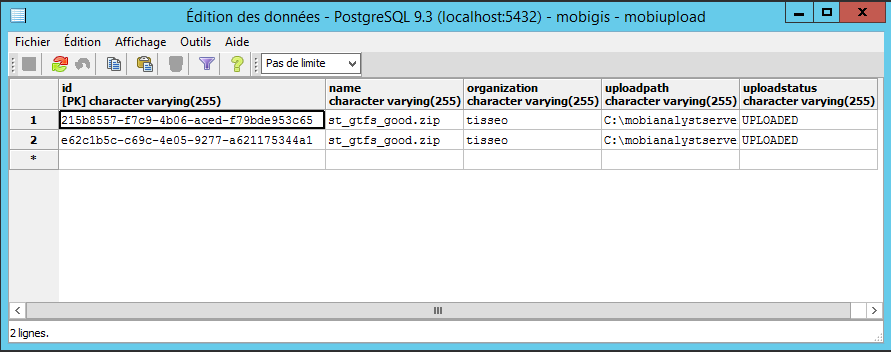
\includegraphics[width=14cm]{images/tablePostgres_mobiupload_small.png}
\caption{\label{TablePostgres}Table des uploads sur le SGBD PostgreSQL}
\end{figure} 

A chaque requête POST du client, je créé une instance d'objet Upload, je saisis les informations dans ma table de suivi, et je stocke les données envoyées sur le serveur. Pour chaque client ou utilisateur, pour chaque type de données, il y a un répertoire personnalisé, chaque upload est "taggé" d'un identifiant unique "UUID".
Le code métier qui a été implémenté est pour le moment le test sur le type de données envoyées, la validation des données et la production d'un rapport d'un validation (JSON), enfin l'extraction (récursive) des données contenues dans l'archive.\\

\subsubsection{Perspectives}



\subsection{DataWizard}

\subsubsection{Présentation : spécifications fonctionnelles}

Le projet "DataWizard" ....\\

\subsubsection{Technologies : spécifications techniques}


\subsubsection{Objectifs / Développements}


\subsubsection{Résultats obtenus / Difficultés rencontrées}


\subsubsection{Perspectives}

